\section{Simulation in LabVIEW}  

\begin{figure}[h!]
\centering
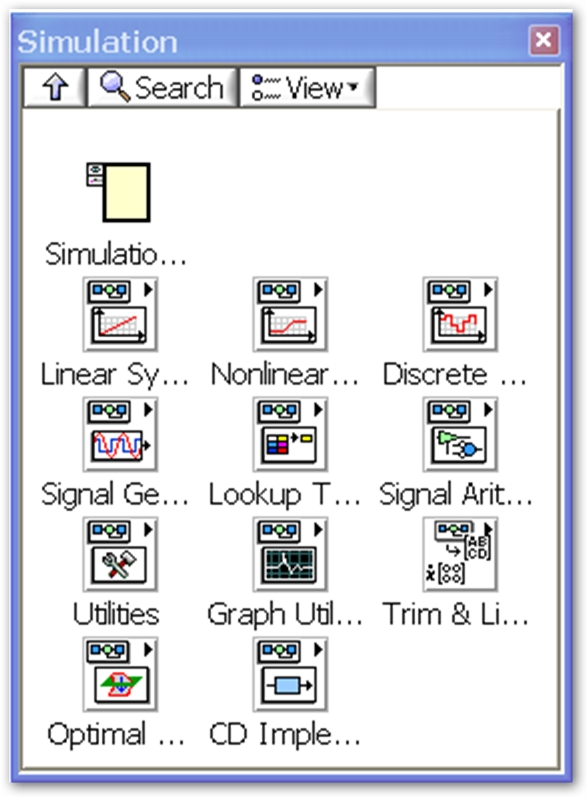
\includegraphics[height=3in]{simulation/palette2}
\caption{The Simulation Pallette}
\label{fig-simulationpallette}
\end{figure}

The ``simulation loop'' will be one of the fundamental tools used in both
simulating systems \emph{and} running hardware-in-the-loop experiments.  It can
be obtained by opening up the simulation palette in the back panel (shown in
Fig.~\ref{fig-simulationpallette}), clicking on the upper left ``simulation
loop'' icon, and dragging it into the back panel.  It may then be stretched to
any desired size.  The result will look something like the loop seen in
Fig.~\ref{fig-simulationloop}.  All the things that need to execute at every
time step in a simulation or hardware experiment should be placed within the
simulation loop.  Everything else can be kept outside of it.  

\begin{figure}[h!]
\centering
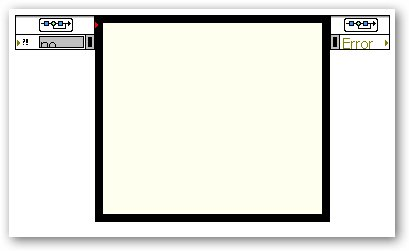
\includegraphics[width=3in]{simulation/simmodsimple}
\caption{The Simulation Loop}
\label{fig-simulationloop}
\end{figure}



The simulation loop determines the
\begin{enumerate}
\item integration algorithm used (e.g., Euler (fixed time step), Runge-Kutta,
  and variable time step algorithms);
\item Determines the step size both for fixed time step integration algorithms
  and for running hardware experiments;
\item length of time for the simulation;
\item timing parameters (involving the clock, an external clock, how fast to
  access said clock, etcetera).  
\end{enumerate}

All these options can be configured by right-clicking on the simulation loop and
selecting Configure Simulation Parameters.  The dialog box is shown in
Fig.\ref{fig-simulationparameters}


\begin{figure}[h!]
\centering
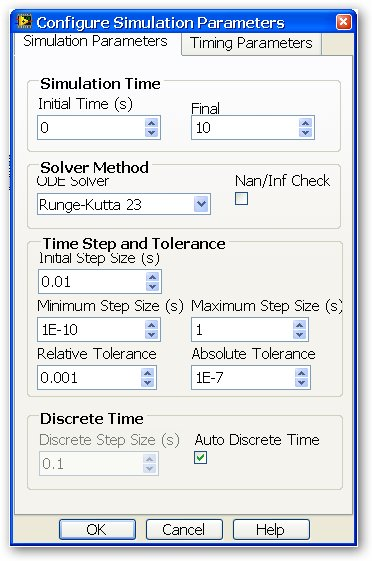
\includegraphics[height=3in]{simulation/simparams}
\caption{A LabVIEW Simulation Loop}
\label{fig-simulationparameters}
\end{figure}


The palettes contain the other operations you may wish to use.  These include:

\begin{enumerate}
\item Generating a signal.  For instance, one can create a step-input from the Signal
Generation pallette.  After placing the step-function in the Simulation Loop,
double click on it.  This will bring up the configuration window.  Within the
configuration window is a list of parameters.  Clicking on any of the parameters
will open ``Parameter Information,'' which allows you to modify the selected
parameter(i.e. final value of step-input = 10).
\item Mathematical operations, such as summation and multiplying a signal by a gain,
can be found in the Signal Arithmetic palette.  Each of these can be
individually configured\textendash for instance, clicking on the summation block in the
panel will allow one to configure it for ``negative'' feedback.  
\item Linear effects, such as time delay are found in the Linear Systems
  palette.  (Note that within LabVIEW, a time delay is know as ``transport
  delay.'')
\item Nonlinear effects such as saturation are found in the Nonlinear Systems
  palette.
\item Graphics: Plots can be generated using Graph Utilities.  In general, you will want to use
a sim-time wave form, but you may wish to use an XY graph if you want trace functionality.  
\end{enumerate}

\begin{figure}[h!]
\centering
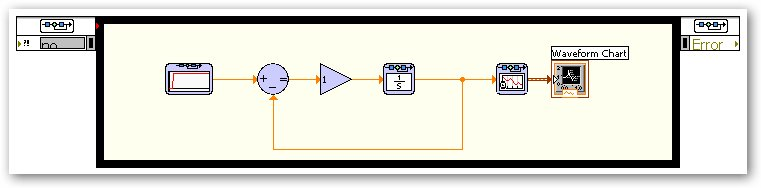
\includegraphics[width=6in]{simulation/simpleloop}
\caption{A simple feedback controller}
\label{fig-simplefeedback}
\end{figure}

\subsection{Creating Sub-Systems in your Simulation}

You will find that your code gets quite complicated as you get more
functionality.  If you want to replace part of your code with a subsystem block,
just select the parts you want in the subsystem and go to \emph{Edit} and select
\emph{Create Simulation Subsystem}.  This will create a block that has the same
inputs and outputs and the region you selected.  You can then view the contents
of the block by right clicking on it and selecting \emph{Open Subsystem}.


More information on the simulation module can be found at \cite{haugen_labview}.






 

%% Local Variables:
%% TeX-master: "../LVmanual.tex"
%% End:

